\documentclass[a4paper]{article}

% Packages
\usepackage[utf8]{inputenc}
\usepackage{geometry}
\geometry{left=1.5cm, right=1.5cm, top=2.54cm, bottom=2.54cm}
\usepackage{graphicx, setspace, amsmath, amssymb, titlesec, fancyhdr, parskip, indentfirst, etoolbox, caption, cite, xcolor}
\usepackage{listings}
\usepackage{url}
\usepackage{hyperref}
\usepackage{multicol}
\usepackage[brazil]{babel}

\addto\captionsbrazil{
  \renewcommand{\refname}{Referências}
}

% Title Formatting
\titleformat{\section}{\centering\large\scshape}{\thesection}{1em}{}
\titleformat{\subsection}{\normalsize\bfseries}{\thesubsection.}{1em}{}

\setstretch{1.0}
\setlength{\parskip}{6pt}

\titlespacing{\section}{0pt}{6pt}{6pt}
\titlespacing{\subsection}{0pt}{6pt}{6pt}
\titlespacing{\subsubsection}{0pt}{6pt}{6pt}

% Document Title
\title{
    \textbf{Grupo 7 - Exercício 1}
}

\date{}

\captionsetup{labelfont={small,sc}, textfont={small,sc}}

% Section Numbering
\renewcommand{\thesection}{\Roman{section}.}
\renewcommand{\thesubsection}{\textit{\Alph{subsection}.}}
\renewcommand{\thesubsubsection}{\textit{\arabic{subsubsection}.}}
\renewcommand{\thetable}{\Roman{table}}
\renewcommand{\thefigure}{\Roman{figure}}

% Make titles italic as well
\titleformat{\subsection}
    {\normalfont\large\itshape}
    {\thesubsection}
    {1em}
    {}

\titleformat{\subsubsection}
    {\normalfont\itshape}
    {\thesubsubsection}
    {1em}
    {}

\setcounter{page}{1}

% Fancy Header Configuration
\pagestyle{fancy}
\fancyhf{}

% First Page Header
\fancypagestyle{firstpage}{
    \fancyhead[C]{
        \centering
        {\fontsize{14pt}{10pt}\selectfont
        \textbf{Universidade de São Paulo}\\[0.5em]
        \textbf{ACH2027 - Gestão de Projetos de Tecnologia da Informação}}\\[0.2em]
        {\fontsize{8pt}{10pt}\selectfont
        \textbf{Prof. Doutor:} Edmir Parada Vasques Prado \hspace{1cm}
        \textbf{Ano:} 2° Semestre/2026}
    }
}

% Default Header for Other Pages
\fancyhead[C]{
    \textbf{Escola de Artes, Ciências e Humanidades - Universidade de São Paulo}
}

\begin{document}

\maketitle
\vspace{-1.5cm}
\thispagestyle{firstpage}

% =========================================================
% INTEGRANTES
% =========================================================

\begin{multicols}{2}
    \centering

    \textbf{Gustavo G. França do Nascimento}\\
    15637551\\
    T94
    
    \vspace{0.5cm}
    
    \textbf{Kauã Lima de Souza}\\
    15674702\\
    T94
    
    \vspace{0.5cm}

    \textbf{Kevin Rodrigues Nunes}\\
    15676030\\
    T94
    
    \vspace{0.5cm}
    
    \textbf{Victor Yodono}\\
    13829040\\
    T94

\end{multicols}

\vspace{-0.2cm} % Ajuste de espaçamento vertical

% =========================================================
% CONTEÚDO
% =========================================================

\singlespacing
\setlength{\parskip}{6pt}
\setlength{\parindent}{0.5cm}

\section{Declaração de Escopo do Projeto}

De acordo com o \textbf{Guia PMBOK} (Capítulo 5 - Gerenciamento do Escopo do Projeto), a Declaração do Escopo do Projeto descreve detalhadamente as entregas do projeto e o trabalho necessário para criá-las. Ela fornece um entendimento comum do escopo entre as partes interessadas e contém as restrições, premissas e exclusões.

Abaixo está a Declaração de Escopo para o \textbf{Sistema de Controle de Acesso da EACH}.

\subsection{Descrição do Escopo do Produto}

Desenvolvimento e implantação de um sistema (software e equipamentos associados) para gerenciar e controlar a entrada e saída de pessoas e veículos nas dependências da EACH. O sistema automatizará o acesso da comunidade acadêmica (docentes, funcionários, alunos) e terceirizados regulares, além de fornecer um módulo para o cadastro, registro e liberação de visitantes. A solução contará com controle de hierarquia de acesso via senha, módulos especiais para gestão de grandes eventos e um painel para geração de relatórios gerenciais e de controle de frequência.

\subsection{Critérios de Aceitação}

Para que o projeto seja considerado concluído e aceito pela Diretoria da unidade, as seguintes condições devem ser atendidas:

\begin{itemize}
    \item \textbf{Funcionais:} O sistema deve liberar o acesso automaticamente para usuários cadastrados (via Nº USP ou CPF) e reter visitantes até que o cadastro seja efetuado.
    \item \textbf{Segurança e Regras:} O acesso ao sistema de gestão deve exigir autenticação por senha e respeitar níveis hierárquicos pré-definidos (ex: administrador, operador de portaria).
    \item \textbf{Desempenho (Relatórios):} O sistema deve ser capaz de emitir, sem falhas, relatórios exatos de frequência de entrada de pessoas (filtrado por Nº USP e CPF) e veículos (filtrado por categoria).
    \item \textbf{Operacionais:} As rotinas especiais (como o pré-cadastramento em lote para eventos de grande porte) devem funcionar adequadamente, sem sobrecarregar a portaria.
    \item \textbf{Cronograma e Custos:} O projeto deve ser totalmente entregue e implantado no prazo máximo de 1 (um) ano, respeitando os limites orçamentários estabelecidos para equipamentos e recursos humanos.
\end{itemize}

\subsection{Entregas do Projeto (Deliverables)}

\begin{itemize}
    \item Documento de Requisitos e Arquitetura do Sistema.
    \item \textbf{Módulo de Controle de Acesso:} Funcionalidades de leitura e liberação de catracas/cancelas para pessoas e veículos.
    \item \textbf{Módulo de Gestão de Usuários e Visitantes:} Interface para cadastro de perfis (docentes, alunos, funcionários, terceirizados e visitantes) e definição de hierarquias de acesso.
    \item \textbf{Módulo de Rotinas Especiais:} Área do sistema dedicada ao pré-cadastro rápido/em lote para grandes eventos.
    \item \textbf{Módulo de Relatórios:} Painel gerador de relatórios de controle e frequência (por Nº USP, CPF e Veículos).
    \item Equipamentos e materiais de controle de acesso (catracas, cancelas, leitores, etc.) comprados, instalados e configurados.
    \item Treinamento para a equipe de operação (portaria/segurança) e administração do sistema.
\end{itemize}

\subsection{Exclusões do Projeto (O que está fora do escopo)}

\begin{itemize}
    \item Controle de acesso interno de portas de salas de aula, laboratórios e gabinetes (o foco é a entrada principal/perímetro da Universidade).
    \item Desenvolvimento de módulos de cobrança (tarifação de estacionamento).
    \item Manutenção e suporte técnico contínuo do sistema após a implantação final e encerramento do projeto.
    \item Sistemas de câmeras de segurança (CFTV) não integrados diretamente à catraca/cancela.
\end{itemize}

\subsection{Restrições (Constraints)}

Limitações impostas ao projeto, relativas a tempo, custo, recursos e regulamentos:

\begin{itemize}
    \item \textbf{Prazo:} A implantação total do sistema não pode ultrapassar 1 (um) ano. O desenvolvimento deve ser finalizado em agosto de 2026.
    \item \textbf{Orçamento (Equipamentos):} O gasto com aquisição de equipamentos e materiais está limitado à faixa de R\$ 300.000,00 a R\$ 600.000,00.
    \item \textbf{Orçamento (Bolsas):} O custo com alunos está restrito ao fornecimento de 5 a 8 bolsas de R\$ 2.000,00 mensais cada, pelo período exato de 6 meses.
    \item \textbf{Recursos Humanos:} O desenvolvimento do sistema é restrito à participação de alunos do último ano de SI (onde a atividade contará como estágio obrigatório) \textbf{OU} à contratação de uma Start-Up da incubadora da EACH.
    \item A equipe exige a presença de um Líder de Projeto subordinado à Diretoria e um Analista de Sistemas Sênior (graduado em SI).
\end{itemize}

\subsection{Premissas (Assumptions)}

Fatores considerados verdadeiros, reais ou certos para fins de planejamento:

\begin{itemize}
    \item A administração da Universidade (USP/EACH) fornecerá acesso seguro e integrado à base de dados atual de docentes, funcionários e alunos (Números USP, CPFs e dados de veículos) para a carga inicial do sistema.
    \item As instâncias acadêmicas competentes aprovarão a participação dos alunos no projeto para validação dos créditos de estágio de graduação a tempo do início em agosto de 2026.
    \item Caso a opção escolhida seja o uso de alunos bolsistas, haverá alunos de SI suficientes, capacitados e interessados no último ano letivo para preencher as 5 a 8 vagas.
    \item A infraestrutura física e de rede da EACH nos pontos de entrada (portarias) suportará a instalação dos novos equipamentos sem necessidade de obras civis complexas e fora do orçamento previsto.
\end{itemize}

\section{Esboço da Estrutura Analítica do Projeto (EAP)}

A Estrutura Analítica do Projeto (EAP) apresenta a decomposição hierárquica do trabalho necessário para atingir os objetivos do projeto. O diagrama a seguir ilustra as principais fases e entregas.

\begin{figure}[p] % O [p] diz ao LaTeX para usar uma página inteira só para figuras
    \centering
    % keepaspectratio impede que a imagem fique esticada/distorcida
    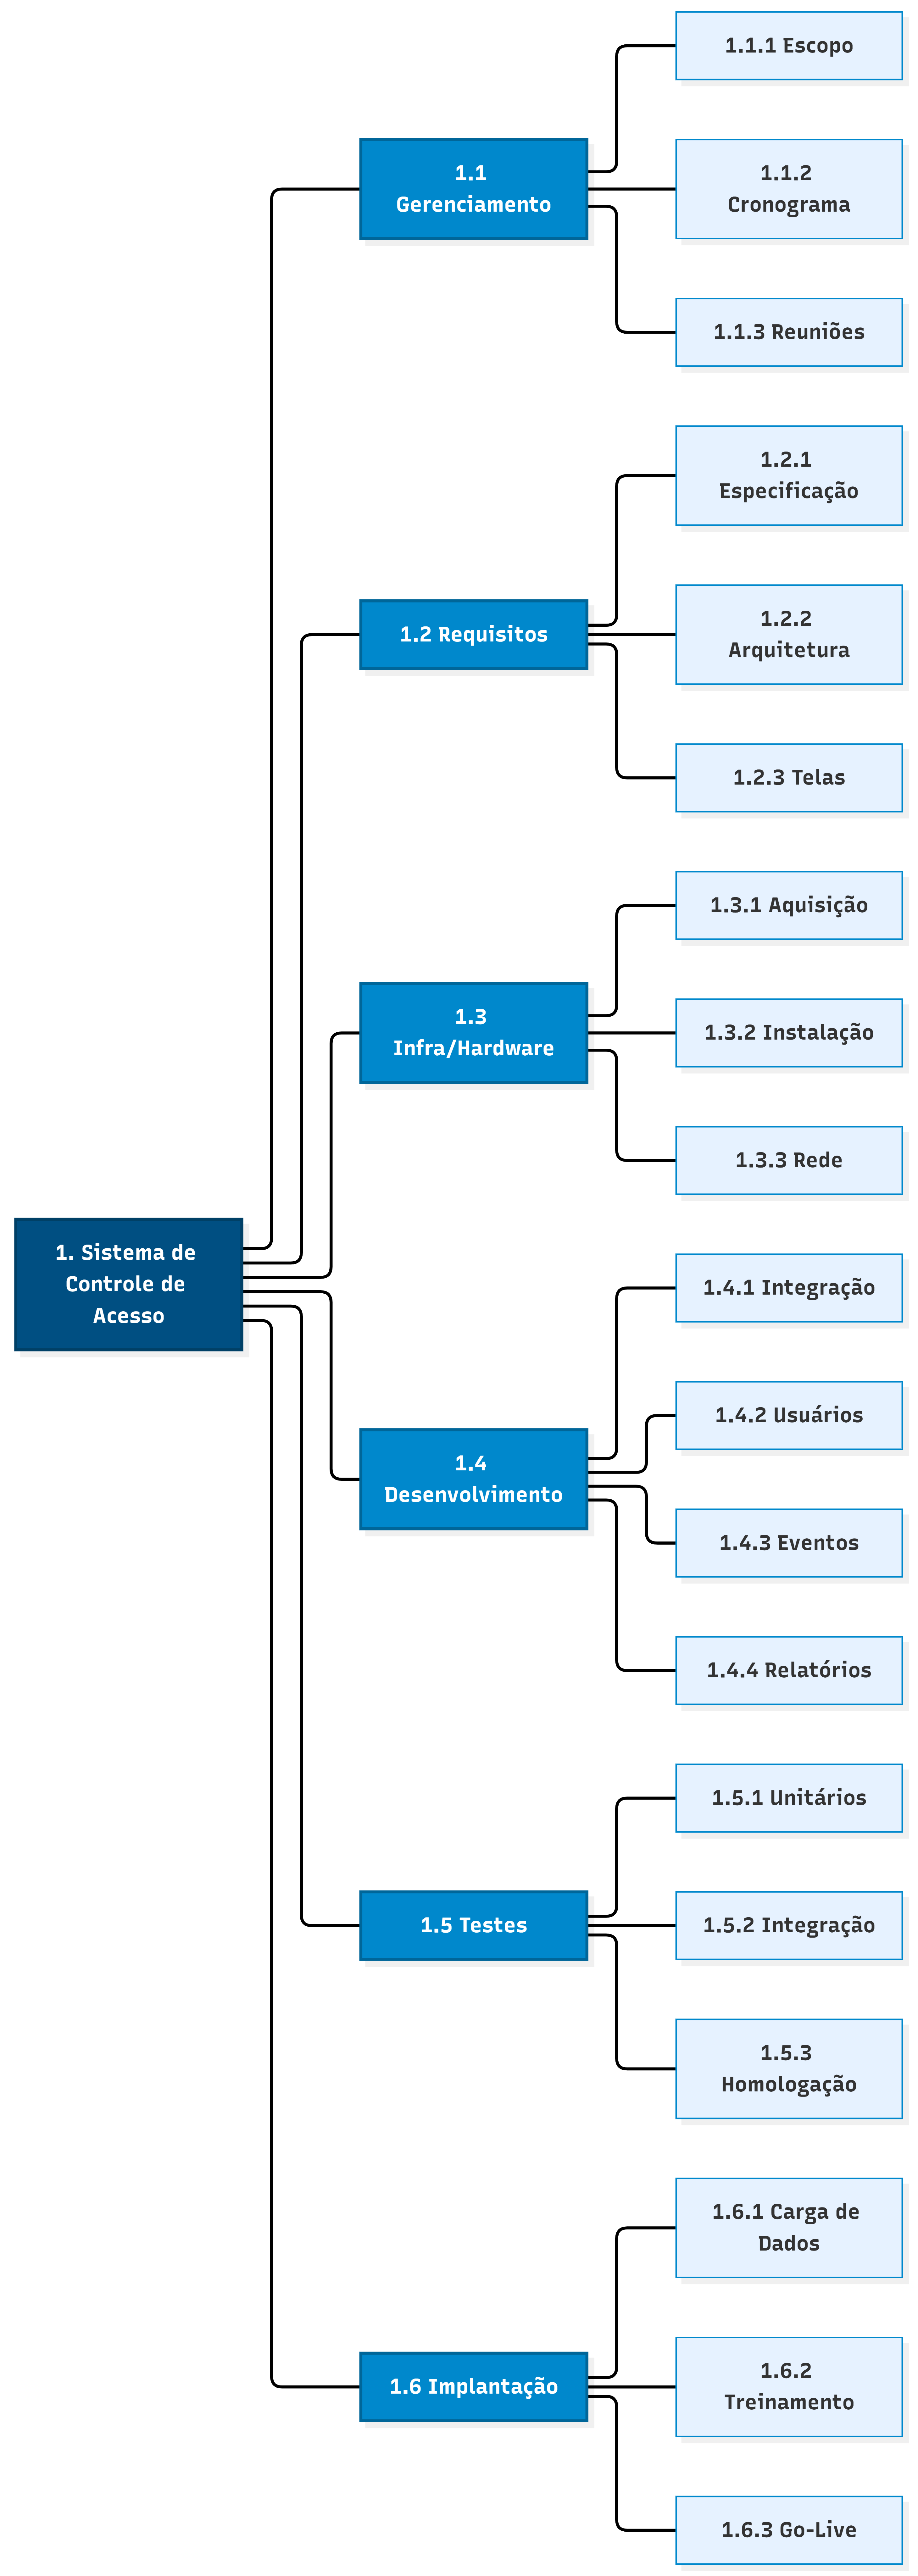
\includegraphics[width=\textwidth, height=0.85\textheight, keepaspectratio]{Sistema de Controle de-2026-09-25-010235.png}
    \caption{Estrutura Analítica do Projeto (EAP)}
    \label{fig:eap}
\end{figure}

\section{Registro de Uso de Inteligência Artificial}

Em conformidade com a Política de Uso de Ferramentas de Inteligência Artificial Generativa da disciplina ACH2027, declaramos explicitamente a utilização de IA como suporte ao aprendizado, ideação e estruturação deste documento.

\begin{table}[htbp]
    \centering
    \renewcommand{\arraystretch}{1.5}
    \small
    \begin{tabular}{|p{3cm}|p{6cm}|p{6cm}|}
        \hline
        \textbf{Registro de Uso de IA} & \textbf{Registro 01: Declaração de Escopo e LaTeX} & \textbf{Registro 02: Diagramação da EAP (Mermaid)} \\
        \hline
        \textbf{Problema / Objetivo} & Elaborar a Declaração de Escopo (PMBOK) a partir do caso semestral da atividade proposta e formatar o conteúdo no template LaTeX do grupo. & Criar o diagrama visual da Estrutura Analítica do Projeto (EAP) e gerar o código exportável para o Overleaf. \\
        \hline
        \textbf{Ferramenta de IA} & Gemini 3.1 Pro (Setembro/2026). & Gemini 3.1 Pro (Setembro/2026). \\
        \hline
        \textbf{Comandos} & "Com base no projeto a seguir, elabore a declaração de escopo... do PMBOK" e "Formate isso no seguinte latex...". & "faça um esboço da estrutura analítica... precisa ser um diagrama" e "me de um mermaid... ficou muito largo horizontalmente". \\
        \hline
        \textbf{Revisão dos resultados} & A primeira versão não abordava detalhes técnicos de software. Perguntamos se era necessário e recebemos um tetalhamento de questões como Open Source e LGPD. Decidimos não incluir, já que a declaração do escopo é uma visão alto nível de gestão. & O formato padrão (Top-Down) do Mermaid extrapolava as margens da página. Ajustamos as instruções para gerar formatos otimizados (Left-Right) adequados ao papel A4 no Overleaf. \\
        \hline
        \textbf{Aplicação no trabalho} & Seção de Declaração de Escopo do Projeto. & Seção da Estrutura Analítica do Projeto (EAP). \\
        \hline
    \end{tabular}
    \caption{Registro de Uso de IA Generativa.}
    \label{tab:uso_ia}
\end{table}

\begin{thebibliography}{99}

\bibitem{pmi2021}
PMI - PROJECT MANAGEMENT INSTITUTE. \textbf{Um Guia do Conhecimento em Gerenciamento de Projetos (Guia PMBOK)}. 7. ed. Pensilvânia: Project Management Institute, 2021.

\end{thebibliography}

\end{document}